\documentclass{article}

\usepackage[utf8]{inputenc}
\usepackage[T1]{fontenc}

\usepackage{geometry}
 \geometry{
 a4paper,
 total={170mm,257mm},
 left=20mm,
 top=20mm,
 }

\setlength{\parskip}{7pt}
\setlength{\parindent}{0pt}

\title{JTAG introduction}
\date{2019-09-13}

\usepackage{hyperref}
\usepackage{listings}
\usepackage{amssymb}
\usepackage{graphicx}
\graphicspath{ {./images/} }

\lstset{
	breaklines=true,
	columns=fullflexible,
	tabsize=4,
	showstringspaces=false,
	frame=single
}

\begin{document}
	\maketitle
	
	\section{About}
	
	JTAG (Joint Test Action Group) is a standard for testing and verifying printed circuit boards.
	
	It allows access to internal registers of a device and has multiple applications: debugging, programming, testing, etc.
	
	\section{Connections}
	
	A JTAG compliant device presents at least one TAP (Test Acces Port). The daisy-chained JTAG (IEEE 1149.1) uses the following signals:
	
	\begin{itemize}
	\item \textbf{TDI}: Test Data In
	\item \textbf{TDO}: Test Data Out
	\item \textbf{TCK}: Test Clock
	\item \textbf{TMS}: Test Mode Select
	\item \textbf{TRST}: Test Reset (optionnal)
	\end{itemize}
	
	\begin{center}
	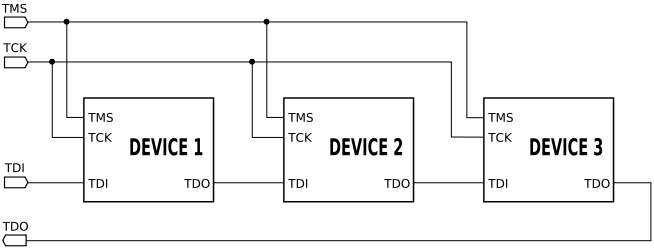
\includegraphics[scale=0.7]{Jtag_chain.png}
	\end{center}
	
	Multiple TAPs can be chained by connecting the TDI and TDO together.
	
	\section{TAP controller}
	
	The behaviour of the JTAG system is controlled by an internal state machine. The transitions are decided by the TMS signal, sampled by the TCK clock.
	
	\begin{center}
	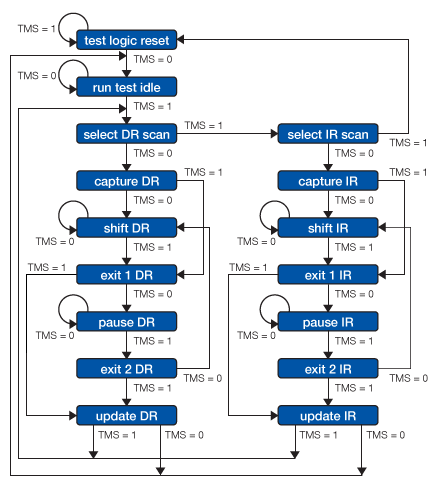
\includegraphics[scale=0.75]{tap_state_machine.png}
	\end{center}
	
	
	\section{Registers and instructions}
	
	Operating the state machine allows accessing the TAP internal registers.
	
	\begin{center}
	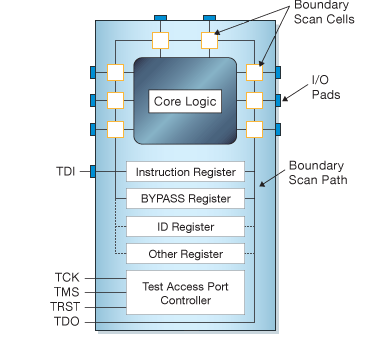
\includegraphics[scale=0.75]{tap.png}
	\end{center}
	
	\subsection{Instruction register}
	
	The instruction register can be small (a few bits, the RISC-V debug specification demands at least 5 bits for example). It contains the opcode of the current instruction. Each instruction can be associated with a data register.
	
	Except for BYPASS and EXTEST, the exact opcodes are defined by the TAP implementor.
	
	The IR is directly manipulated by the state machine and other data registers are accessed through it.
	
	\subsection{IDCODE}
	
	This instruction is associated with a 32-bit register which contains a manufacturer code, a part number and a part version code.
	
	\subsection{BYPASS}
	
	An opcode of all ones must implement this instruction.
	
	The associated register is only 1-bit wide and has no effect. It is used to bypass the TAP.
	
	\subsection{Other}
	
	Other instructions and associated registers can be defined by the TAP implementor, so other features can be implemented, like debugging or data access.
	
	These instructions are specific to each device.
	
	\subsection{Boundary scan}
	
	A TAP may or may not implement the Boundary Scan feature.
	
	The boudary scan cells and some instructions provide access to the device's I/Os in a path around the device's boundary. It is possible to read and write the values of individual pins.
	
	\section{In practice}
	
	\subsection{Connectors}
	
	There is no standard JTAG connector. Existing connectors depend on the manufacturer. They have various pinouts, forms, and sizes.
	
	\begin{center}
	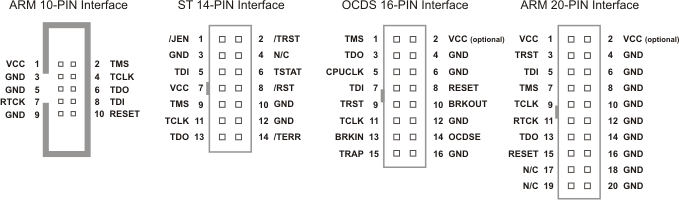
\includegraphics[scale=2]{jtag_connectors.png}
	\end{center}
	
	\subsection{USB}
	
	It is possible to use USB to access a JTAG scan chain. The converter circuitry can be mounted on the cable or integrated in the PCB.
	
	\subsection{Bit banging}
	
	Due to the low complexity of the TAP controller state machine, it is possible to bit-bang the JTAG interface. OpenOCD has a \textit{sysfsgpio} driver that does it using gpio lines via sysfs.
	
	\section{References}
	
	\url{https://en.wikipedia.org/wiki/JTAG}
	
	\url{https://standards.ieee.org/standard/1149_1-2013.html}
	
	\url{https://www.xjtag.com/about-jtag/jtag-a-technical-overview/}
	
	\url{https://blog.senr.io/blog/jtag-explained}
	
	\url{http://openocd.org/doc/doxygen/html/sysfsgpio_8c.html#details}
	
	
\end{document}
